\documentclass{beamer}

\input{../ts-glærur}

\title{FOR3R - Gagnagrindur}

\begin{document}
\begin{frame}
\titlepage
\end{frame}

\begin{frame}{Gagnagrindur}

\begin{quote}
``Smart data structures and dumb code works a lot better than the other way around.''
\end{quote}

\begin{itemize}
 \item Það hvernig geyma má og vinna með gögn er stórt atriði innan tölvunarfræðinnar
 \item Við höfum skoðað röðunarverkefnið fyrir fylki (e. \emph{array}) ítarlega
 \item Mörg merkileg reiknirit virka á aðrar gagnagrindur (e. \emph{data structure}, sh. \emph{gagnaskipan}) en fylki
 \begin{itemize}
  \item Sum reiknirit verða mun skýrari þegar þau eru byggð á góðri gagnagrind
 \end{itemize}
\end{itemize}
\end{frame}

\section{Fylki}
\begin{frame}{Fylki}
\begin{itemize}
 \item Hefðbundin útfærsla á fylki: Samfelld, minnisblokk af fastri stærð sem inniheldur einsleit stök
 \begin{itemize}
  \item Fylki hefur lykla sem notaðir eru til að vísa í stökin
  \item Fyrsta stakið hefur (oftast) lykilinn 0
  \item Önnur stök fá númer eftir fjarlægð (e. \emph{offset}) frá fyrsta stakinu
 \end{itemize}
 \item Kostir og gallar:
 \begin{itemize}
  \item Einfaldur og hraðvirkur aðgangur að minni
  \item Gefur lítinn strúktur, stærðartakmarkanir, þarf samfellt minni, gagnaeyðingar geta verið tímafrekar
 \end{itemize}
\end{itemize}
\end{frame}

\section{Listar}
\begin{frame}{Listar}
\begin{itemize}
 \item Listi er \emph{röð} af gögnum
 \item Ekki er hægt að nálgast gögn í lista nema með því að ferðast í gegnum listann
 \begin{itemize}
  \item Ekkert ``random access''
  \item Þurfum að nota ítrun (e. \emph{iteration})
 \end{itemize}
\end{itemize}
\end{frame}

\begin{frame}{Notkun á orðunum ``listi'' og ``fylki''}
\begin{itemize}
 \item Í daglegu tali eru orðin listi (e. \emph{list}) og fylki oft notuð jöfnum höndum
 \begin{itemize}
  \item Höfum gerst sek um það í þessum áfanga
 \end{itemize}
 \item Þetta er mögulega vegna þess að æðri forritunarmál (e. \emph{high level programming languages}) eru oft með flóknar gagnagrindur sem eiga að sameina kosti lista og fylkja
 \begin{itemize}
  \item \href{https://docs.python.org/3.5/faq/design.html\#how-are-lists-implemented}{Í Python} er ``list'' í rauninni fylki 
  \item Ku vera svipað í C\# (\texttt{List<T>}) og Java (\texttt{ArrayList<T>})
 \end{itemize}
\end{itemize}

\end{frame}


\begin{frame}{Listaútfærslur}
\begin{itemize}
 \item Venjuleg útfærsla á listum er svokallaður tengdur listi (e. \emph{ linked list})
 \item Tengdur listi samanstendur af einum eða fleiri hnútum (e. \emph{nodes}) og tengingum þar á milli
 \begin{itemize}
  \item Hnúturinn inniheldur þá gögn
 \end{itemize}
 \item Tvær aðalútfærslur: Tvítengdur listi (e. \emph{doubly linked list}) og eintengdur listi (e. \emph{singly linked list})
 \begin{itemize}
  \item Í tvítengdum lista inniheldur hver hnútur gögn, vísun í næsta hnút og vísun í hnútinn á undan
  \item Í eintengdum lista er vísun í hnútinn á undan sleppt
 \end{itemize}
\end{itemize}
\end{frame}

\begin{frame}{Tengdir listar}
\begin{center}
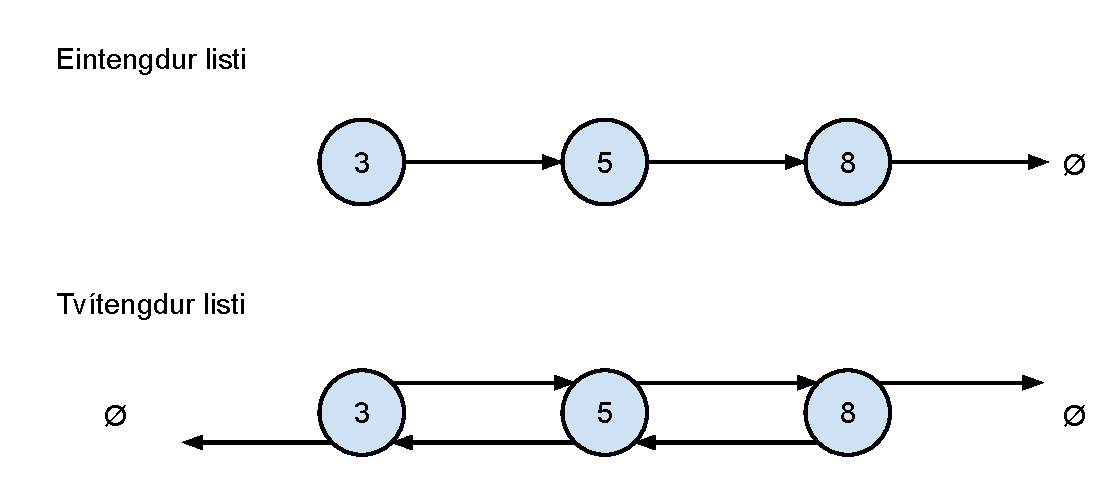
\includegraphics[width=\textwidth]{Pics/listar}
\end{center}
\end{frame}

\section{Dictionary}
\begin{frame}{Dictionary}
\begin{itemize}
 \item Sjáum fyrir okkur almennari leið til að tengja saman lykla og gildi
 \begin{itemize}
  \item Í fylkjum eru lyklarnir tölur, í röð
  \item Hvað ef við getum notað hvaða (föst) gildi sem er sem lykla?
 \end{itemize}
 \item Slík gagnagrind er til í Python, kölluð dictionary (\texttt{dict})
 \begin{itemize}
  \item Útfærð með hakkatöflu (e. \emph{hash table})
 \end{itemize}
 \item Python dictionaries eru dæmi um svokallaða vörpun (e. \emph{map})
\end{itemize}
\end{frame}

\begin{frame}[fragile]{Dictionary í Python}
Dæmi um aðgerðir með dictionary:
\begin{minted}{python}
>>> dict1 = {} # tómt dictionary
>>> dict2 = {"lykill1" : "gildi1"} # nýtt dict með gildi
>>> dict2["lykill2"] = "gildi2" # innsetning
>>> del dict2["lykill2"] # eyðing
>>> dict2["lykill1"] = "nýtt gildi" #breyting á gildi
>>> dict2["lykill1"] #uppfletting
'nýtt gildi'
\end{minted}
\end{frame}

\section{Forritun}

\begin{frame}{Að skrifa nýja gagnagrind}
\begin{itemize}
 \item Forritunarmál eru með innbyggðar gagnagrindur
 \begin{itemize}
  \item Getum notað þær til að smíða
 \end{itemize}
 \item Stundum höfum við ``einungis'' benda og fylki
 \item Hlutbundin forritun getur verið öflugt tól
\end{itemize}
\end{frame}

\section{Tré}

\begin{frame}{Tré}
\begin{columns}[c]
\column{0.7\textwidth}
\begin{itemize}
 \item Hægt er að nota hnúta til að útfæra ýmsar gagnagrindur
 \begin{itemize}
  \item Dæmi um slíkt eru tvíundartré
 \end{itemize}
  \item Hnútur í tvíundartré inniheldur gögn, vísun í ``vinstri'' hnút og ``hægri'' hnút
 \begin{itemize}
  \item Vinstri og hægri hnútarnir eru kallaðir ``börn'' hnútarins
 \end{itemize}
 \item Einn hnútur gegnir hlutverki rótar (e. \emph{root})
 \item Hnútar sem eiga engin börn eru kölluð ``lauf'' (e. \emph{leaves})
\end{itemize}
\column{0.3\textwidth}
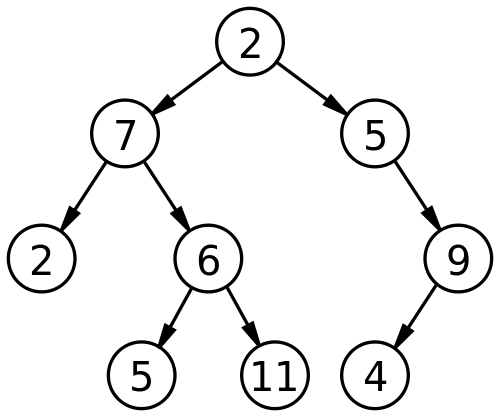
\includegraphics[width=\linewidth]{Pics/binary-tree}
\end{columns}
\end{frame}

\begin{frame}[fragile]{Að skrifa nýja gagnagrind}
Möguleg útfærsla á hnút í tvíundartré er eftirfarandi:
\begin{minted}{python}
class TreeNode:
    def __init__(self, data, left=null, right=null):
        self.data = data
        self.left = left
        self.right = right
\end{minted}

left og right væru hér líka hnútar.
\end{frame}


\begin{frame}
\begin{itemize}
 \item Næst:
 \begin{itemize}
  \item Meira um tré
  \item Biðraðir, hlaðar og forgangsbiðraðir
  \item Almenn net
 \end{itemize}
\end{itemize}
\end{frame}


\end{document}
